\chapter{Fourier Transform }
\section{Integral Transforms}
Frequently in mathematical physics we encounter pairs of functions related by an expression of the form
\begin{equation}
g(x)=\int_{a}^{b} f(t) K(x, t) d t\label{FT-01}
\end{equation}
where it is understood that $a, b$, and $K(x, t)$ (called the kernel) will be the same for all function pairs $f$ and $g$. We can write the relationship expressed in Eq. (\ref{FT-01}) in the more symbolic form
\begin{equation}
g(x)=\mathcal{L} f(t)
\end{equation}
thereby emphasizing the fact that Eq. $(\ref{FT-01})$ can be interpreted as an operator equation. The function $g(x)$ is called the integral transform of $f(t)$ by the operator $\mathcal{L}$, with the specific transform determined by the choice of $a, b$, and $K(x, t)$. The operator defined by Eq. (\ref{FT-01}) will be linear:
\begin{align}
\int_{a}^{b}\left[f_{1}(t)+f_{2}(t)\right] K(x, t) d t&=\int_{a}^{b} f_{1}(t) K(x, t) d t+\int_{a}^{b} f_{2}(t) K(t) d t \\
\int_{a}^{b} c f(t) K(\alpha, t) d t&=c \int_{a}^{b} f(t) K(\alpha, t) d t
\end{align}
In order for transforms to be useful, we will shortly see that we need to be able to "undo" their effect. From a practical viewpoint, this means that not only must there exist an operator $\mathcal{L}^{-1}$, but also that we have a reasonably convenient and powerful method of evaluating
\begin{equation}
\mathcal{L}^{-1} g(x)=f(t)
\end{equation}
for an acceptably broad range of $g(x)$. The procedure for inverting a transform takes a wide variety of forms that depend on the specific properties of $K(x, t)$, so we cannot write a formula that is as general as that for $\mathcal{L}$ in Eq. (\ref{FT-01}).\\
Not all superficially reasonable choices for the kernel $K(x, t)$ will lead to operators $\mathcal{L}$ that have inverses, and even for strategically chosen kernels it may be the case that $\mathcal{L}$ and $\mathcal{L}^{-1}$ will only exist for substantially restricted classes of functions. Thus, the entire development of the present chapter is restricted (for any given integral transform) to functions for which the indicated operations can be carried out.\\
Before embarking on a study of integral transforms, we may well ask, "Why are integral transforms useful?" Their most common applications are in situations illustrated schematically in Fig. 20.1, where we have a problem that can be solved only with difficulty, if at all, in its original formulation (usually in ordinary space, sometimes called \textbf{direct }or \textbf{physical space}). However, it may happen that the transform of the problem can be solved relatively easily. Our strategy, then, will be to formulate and solve our problem in the transform space, after which we transform the solution back to direct space. This strategy often works because the most popular integral transforms are changed in simple ways by differentiation and integration operators, with the result that differential and integral equations assume relatively simple forms. This feature will be discussed and illustrated at length later in this chapter.\\
Another frequent use of integral transforms is to use one, together with its inverse, to form an \textbf{integral representation} of a function that we originally had in an explicit form. This move (which appears to be in the direction of generating greater complexity) has value that arises from the relatively simple behavior of the transforms of differentiation and integration operators. Procedures involving integral representations are also presented in later sections of this chapter.
\begin{figure}[H]
	\centering
	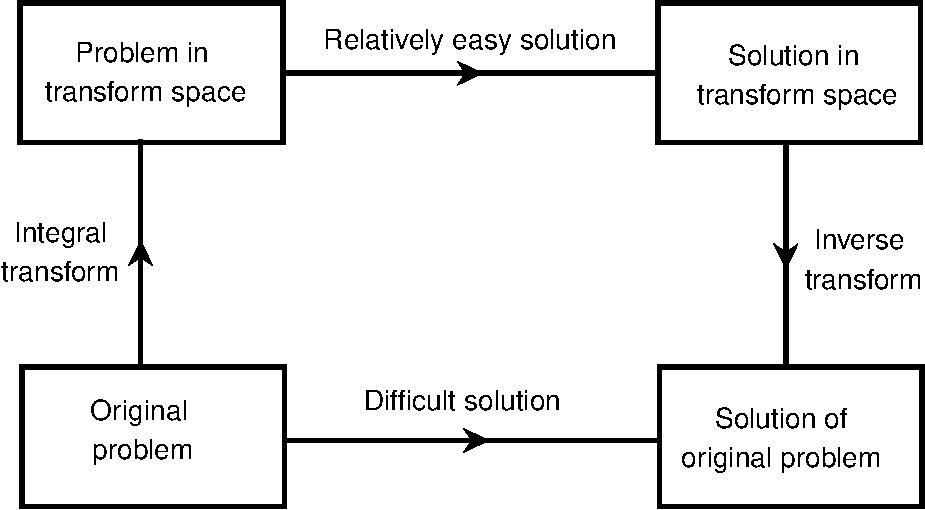
\includegraphics[height=5cm,width=9cm]{FT-01}
\end{figure}
\section{Some Important Transforms}
The integral transform that has seen the widest use is the Fourier transform, defined as
\begin{equation}
g(\omega)=\frac{1}{\sqrt{2 \pi}} \int_{-\infty}^{\infty} f(t) e^{i \omega t} d t
\end{equation}
The notation for this transform is not entirely universal; some writers omit the prefactor $1 / \sqrt{2 \pi}$; we keep it because it causes the transform and its inverse to have formulas that are more symmetrical. In applications involving periodic systems, one occasionally encounters a definition with kernel $\exp \left(2 \pi i \omega t / a_{0}\right)$, where $a_{0}$ is a lattice constant. These differences in notation do not change the mathematics, but cause formulas to differ by powers of $2 \pi$ or $a_{0}$. Caution is therefore advised when combining material from different sources.\\
We have defined the Fourier transform in a notation that assigns the symbol $\omega$ to the transform variable. We did so because, in studying signal processing (an important use of Fourier transforms), the function $f(t)$ usually represents the time behavior of a signal (typically a wave distribution of some kind). Its Fourier transform, $g(\omega)$, can then be identified as the corresponding frequency distribution. However, it is worth pointing out that Fourier transforms turn up in contexts far removed from signal-processing problems; they can be used to advantage in evaluating integrals, in alternative formulations of quantum mechanics, and in a wide range of other mathematical procedures.\\
A second transform that has historically been of great importance is the \textbf{Laplace transform,}
\begin{equation}
F(s)=\int_{0}^{\infty} e^{-t s} f(t) d t .
\end{equation}
One of its useful features is the fact that under transformation, differential equations become algebraic equations. Since algebraic equations are usually easier to solve than differential equations, this feature lends itself to the strategy illustrated. A disadvantage of the Laplace transform is that the formula for its inverse is relatively difficult to use. Historically, this difficulty was dealt with by developing tables of Laplace transforms.
\section{Infinite Fourier Transform}
\begin{align*}
\text{The fourier transform of }f(x)[-\infty<x<\infty] &:\\
f(s)=F\{f(x)\}&=\frac{1}{\sqrt{2 \pi}} \int_{-\infty}^{\infty} f(x) e^{i s x} d x\\
\text{Inverse fourier transform of }f(s)[-\infty<x<\infty] &:\\
f(x)=F^{-1}\{f(s)\}&=\frac{1}{\sqrt{2 \pi}} \int_{-\infty}^{\infty} f(s) e^{-i s x} d s .
\end{align*}
\section{Fourier Sine Transform}
\begin{align*}
f_{s}(\mathrm{~s})&=F_{s}\{f(x)\}=\sqrt{\frac{2}{\pi}} \int_{0}^{\infty} f(x) \sin s x d x \\
f(x)&=F_{s}^{-1}\left\{f_{s}(s)\right\}=\sqrt{\frac{2}{\pi}} \int_{0}^{\infty} f_{s}(s) \sin s x d s
\end{align*}
\section{Fourier Cosine Transform}
\begin{align*}
f_{c}(s)&=F_{c}\{f(x)\}=\sqrt{\frac{2}{\pi}} \int_{0}^{\infty} f(x) \cos s x d x \\
f(x)&=F_{c}^{-1}\left\{f_{c}(s)\right\}=\sqrt{\frac{2}{\pi}} \int_{0}^{\infty} f_{c}(s) \cos s x d s
\end{align*}
\textbf{Important Formula:}\\
\renewcommand*{\arraystretch}{2}
\begin{tabular}{p{5cm}p{5cm}p{6cm}}
	(i) $\int_{0}^{\infty} \frac{\sin a x}{x} d x=\frac{\pi}{2}$&
	(ii) $\int_{0}^{\infty} e^{-x^{2}} d x=\sqrt{\frac{\pi}{2}}$&
	(iii) $\int_{0}^{\infty} e^{-a x} \sin b x d x=\frac{b}{a^{2}+b^{2}}$\\
	(iv) $\int_{0}^{\infty} e^{-a x} \cos b x d x=\frac{a}{a^{2}+b^{2}}$&
	(v) $\int_{0}^{\infty} e^{-a x^{2}} d x=\frac{1}{2} \sqrt{\frac{\pi}{a}}$&
	(vi) $\int_{0}^{\infty} e^{-a x^{2}} \cos b x d x=\frac{1}{2} \sqrt{\frac{\pi}{a}} e^{-b^{2} / 4 a}$\\
	(vii)
	$\int_{-\infty}^{\infty} e^{-a x^{2}+b x} d x=\sqrt{\frac{\pi}{a}} e^{b^{2} / 4 a}$& & 
\end{tabular}
\begin{exercise}
	Find the fourier transform of Gaussian distribution function $f(x)=N e^{-a x^{2}}$ where $N$ and 'a' are constant.
\end{exercise}
\begin{answer}
	\begin{align*}
	F\{f(x)\}=\frac{1}{\sqrt{2 \pi}} \int_{-\infty}^{\infty} f(x) e^{i k x} d x=\frac{1}{\sqrt{2 \pi}} \int_{-\infty} N e^{-a x^{2}} e^{i k x} d x=\frac{N}{\sqrt{2 \pi}} e^{-k^{2} / 4 a}
	\end{align*}
\end{answer}
\begin{exercise}
	Find $F\{\delta(x)\}$
\end{exercise}
\begin{answer}
	\begin{align*}
	F\{f(x)\}=\frac{1}{\sqrt{2 \pi}} \int_{-\infty}^{\infty} f(x) e^{i k x} d x=\frac{1}{\sqrt{2 \pi}} \int_{-\infty}^{\infty} \delta(x) e^{i k x} d x=\frac{1}{\sqrt{2 \pi}}\left[\mathrm{e}^{i k x}\right]_{x=0}=\frac{1}{\sqrt{2 \pi}}
	\end{align*}
\end{answer}
\begin{exercise}
	Find the fourier transform of $f(x)=e^{-a|x|} \quad(-\infty<x<\infty) \quad(a>0)$
\end{exercise}
\begin{answer}
	\begin{align*}
	\begin{aligned}
	F\left[e^{-a|x|}\right] &=\frac{1}{\sqrt{2 \pi}}\left[\int_{-\infty}^{0} e^{a x} e^{i s x} d x+\int_{0}^{\infty} e^{-a x} e^{i s x} d x\right]=\frac{1}{\sqrt{2 \pi}}\left[\left(\frac{e^{(a+i s) x}}{(a+i s)}\right)_{-\infty}^{0}+\left(\frac{e^{-(a-i s) x}}{(i s-a)}\right)_{0}^{\infty}\right] \\
	&=\frac{1}{\sqrt{2 \pi}}\left[\frac{1}{a+i s}+\frac{1}{a-i s}\right]=\frac{2 a}{\sqrt{2 \pi}\left(s^{2}+a^{2}\right)} \because
	\end{aligned}
	\end{align*}
\end{answer}
\begin{exercise}
	If $F\left\{e^{-i 2 \text { avat }}\right\}=f(\omega+a)$, then $F(\cos 2 \pi v a t)=$ ?
\end{exercise}
\begin{answer}
	\begin{align*}
	\mathrm{F}[\cos 2 \pi v \mathrm{vat}]=\mathrm{F} \frac{\left[\mathrm{e}^{\mathrm{i} 2 \pi \mathrm{vat}}+\mathrm{e}^{-\mathrm{i} 2 \pi \mathrm{vat}}\right]}{2}=\frac{1}{2}\left\{F\left[e^{i 2 \pi v a t}\right]+F\left[e^{-i 2 \pi v a t}\right]\right\}=\frac{1}{2}[f(\omega-a)+f(\omega+a)]
	\end{align*}
\end{answer}
\begin{exercise}
	Given that $F[\delta(x-a)]=\exp [-i 2 \pi v a]$, then $F^{-1}[\cos 2 \pi v a]=$ ?
\end{exercise}
\begin{answer}
	\begin{align*}
\text{	As }\quad F\{\delta(x-a)\}&=\exp [-i 2 \pi v a] \quad \Rightarrow \delta(x-a)=F^{-1}[\exp (-i 2 \pi v a)]\\
	\text{Now }F^{-1}(\cos 2 \pi v a)&=F^{-1}\left[\frac{\exp (-i 2 \pi v a)+\exp (i 2 \pi v a)}{2}\right]=\frac{1}{2}[\delta(x+a)+\delta(x-a)]
	\end{align*}
\end{answer}
\begin{exercise}
	Find the fourier cosine transform of the function $f(x)=e^{-a^{2} x^{2}}$
\end{exercise}
\begin{answer}
	\begin{align*}
	\begin{aligned}
	f_{c}(s) &=F_{c}[f(x)]=\sqrt{\frac{2}{\pi}} \int_{b}^{\infty} e^{-a^{2} x^{2}} \cos s x d x=\frac{1}{2} \sqrt{\frac{2}{\pi}} \int_{-\infty}^{\infty} e^{-a^{2} x^{2}} \cos s x d x \\
	&=\frac{1}{2} \sqrt{\frac{2}{\pi}} \text { Real part of } \int_{-\infty}^{\infty} e^{-a^{2} x^{2}} e^{i s x} d x=\frac{1}{2} \sqrt{\frac{2}{\pi}} \text { Real part of }\left(\sqrt{\frac{\pi}{a^{2}}} e^{\frac{i^{2} s^{2}}{4 a^{2}}}\right)=\frac{1}{\sqrt{2 a^{2}}} e^{-s^{2} / 4 a^{2}}
	\end{aligned}
	\end{align*}
\end{answer}
\section{Properties of Fourier Transform}
(i) Linearity theorem: If $F(x)=a_{1} f_{1}(x)+a_{2} f_{2}(x)+\ldots$ then, $f(s)=F[f(x)]=a_{1} f_{1}(s)+a_{2} f_{2}(s)+\ldots$\\
(ii) Change of scale property: If $F[f(x)]=f(s)$, then $F\{f(a x)\}=\frac{1}{a} f(\mathrm{~s} / a)$\\
(iii) If $F\{f(x)\}=f(s)$, then $F\left\{f^{*}(x)\right\}=f^{*}(-s)$\\
(iv) Shifting property: If $f(s)$ is the Fourier transform of $\mathrm{f}(\mathrm{x})$, then $F\{f(x \pm a)\}=e^{\mp i s a} f(s)$\\
(v) Modulation theorem: If $F\{f(x)\}=f(s)$, then $F\{f(x) \cos a x\}=\frac{1}{2} f(s-a)+\frac{1}{2} f(s+a)$
\section{Parseval Identity for Fourier Transform}
If the Fourier transform of $f(x)$ and $g(x)$ be $f(s) \& g(s)$ respectively, then\\
(i) $\int_{-\infty}^{\infty} f(s) g^{*}(s) d s=\int_{-\infty}^{\infty} f(x) g^{*}(x) d x$\\
where $g^{*}(s)$ is complex conjugate of $g(s)$ and $g^{*}(x)$ is the complex conjugate of $g(x)$.\\
(ii) $\left.\int_{-\infty}^{\infty}|f(s)|\right|^{2} d s=\int_{-\infty}^{\infty}|f(x)|^{2} d x$
\begin{exercise}
	(a) Find fourier transform of $f(x)= \begin{cases}1 & \text { for }|x|<a \\ 0 & \text { for }|x|>a\end{cases}$\\
	(b) Using parsevàl's identity show that $\int_{b}^{\infty}\left(\frac{\sin x}{x}\right)^{2} d x=\pi / 2$
\end{exercise}
\begin{answer}
	\begin{align*}
	F\{f(x)\}&=\frac{1}{\sqrt{2 \pi}} \int_{-\infty}^{\infty} f(x) e^{i x x} d x=\sqrt{\frac{2}{\pi}} \frac{\sin a s}{s}\\
	\text{Using parseval identity, }&\int_{-\infty}^{\infty}|f(x)|^{2} d x=\int_{-\infty}^{\infty}|f(s)|^{2} d s\\
	\Rightarrow \quad \int_{-a}^{\infty} l^{2} d x&=\int_{-\infty}^{\infty} \frac{2}{\pi} \frac{\sin ^{2} a s}{s^{2}} d s \quad \Rightarrow \quad 2 a=\frac{2}{\pi} \int_{-\infty}^{\infty}\left(\frac{\sin a s}{s}\right)^{2} d s\\
	\text{Putting }a s&=x \Rightarrow a d s=d x\\
	\Rightarrow \pi&=\int_{-\infty}^{\infty}\left(\frac{\sin x}{x}\right)^{2} d x \quad \Rightarrow \int_{0}^{\infty}\left(\frac{\sin x}{x}\right)^{2} d x=\frac{\pi}{2}
	\end{align*}
\end{answer}
\begin{exercise}
	If the fourier transform of $f(x)$ is $f(s)$, then find the fourier transform of $\frac{d f}{d x}$
\end{exercise}
\begin{answer}
	\begin{align*}
	F\left[\frac{d f}{d x}\right]&=\frac{1}{\sqrt{2 \pi}} \int_{-\infty}^{\infty} \frac{d f}{d x} e^{i x x} d x=\frac{1}{\sqrt{2 \pi}}\left[e^{i x x} f(x)\right]_{-\infty}^{\infty}-\frac{1}{\sqrt{2 \pi}} \int_{-\infty}^{\infty} i s e^{i s x} f(x) d x\\
	\intertext{Since $f(x)$ should be a well behave function for the fourier tranform to exist, therefore, the first term of the above equation should be equal to zero.}
	\text{Then }F\left[\frac{d f}{d x}\right]&=-i s \frac{1}{\sqrt{2 \pi}} \int_{-\infty}^{\infty} e^{i s x} f(x) d x=-\operatorname{isf}(\mathrm{s})
	\end{align*}
\end{answer}
\begin{exercise}
	Find Fourier transform of $f(x)= \begin{cases}x^{2}, & |x|<a \\ 0, & |x|>a\end{cases}$
\end{exercise}
\begin{answer}
	\begin{align*}
	\begin{aligned}
	F\{f(x)\} &=\frac{1}{\sqrt{2 \pi}} \int_{-\infty}^{\infty} e^{i s x} f(x) d x=\frac{1}{\sqrt{2 \pi}} \int_{-a}^{a} e^{i s x} x^{2} d x \\
	&=\frac{1}{\sqrt{2 \pi}}\left[\left(\frac{e^{i s x}}{i s} \cdot x^{2}\right)_{x=-a}^{a}-\frac{2}{i s} \int_{-a}^{a} x e^{i s x} d x\right] \\
	&=\frac{1}{\sqrt{2 \pi}}\left[\frac{a^{2}}{i s}\left(e^{i s a}-e^{-i s a}\right)-\frac{2}{i s}\left[\left(\frac{x e^{i s x}}{i s}\right)_{x=-a}^{a}-\frac{1}{i s} \int_{-a}^{a} e^{i s x} d x\right]\right]
	\end{aligned}
	\end{align*}
\end{answer}
\begin{exercise}
	Find the complex fourier transform $e^{-|x|}$
\end{exercise}
\begin{answer}
	\begin{align*}
	F\left\{e^{-|x|}\right\}&=\frac{1}{\sqrt{2 \pi}} \int_{-\infty}^{\infty} e^{-|x|} e^{i s x} d x=\frac{1}{\sqrt{2 \pi}}\left[\int_{-\infty}^{0} e^{-|x|} e^{i s x} d x+\int_{0}^{\infty} e^{-|x|} \cdot e^{i s x} d x\right]\\
	&=\frac{1}{\sqrt{2 \pi}}\left[\int_{-\infty}^{0} e^{x} \cdot e^{i s x} d x+\int_{0}^{\infty} e^{-x(1-i s)} d x\right]=\frac{1}{\sqrt{2 \pi}}\left[\left[\frac{e^{x(1+i s)}}{1+i s}\right]_{x=-\infty}^{0}+\left[\frac{e^{-x(1-i s)}}{-(1-i s)}\right]_{x=0}^{\infty}\right] \\
	&=\frac{1}{\sqrt{2 \pi}}\left[\frac{1}{1-i s}+\frac{1}{1+i s}\right]=\frac{1}{\sqrt{2 \pi}}\left(\frac{2}{1+s^{2}}\right)
	\end{align*}
\end{answer}
\begin{exercise}
	Find the sine transform of $\frac{x}{1+x^{2}}$
\end{exercise}
\begin{answer}
	\begin{align}
	\text { Firstly we shall determine}&\text{ cosine transform of } \frac{1}{1+x^{2}}\notag\\
	F_{c}\left\{\frac{1}{1+x^{2}}\right\}&=\int_{0}^{\infty} \frac{\cos s x}{1+x^{2}} d x=I(\text { say })\notag\\
	\text{then }I&=\int_{0}^{\infty} \frac{\cos s x}{1+x^{2}} d x\label{FT-03}\\
	\text{Dufferentiating w.r.t.s,}\notag\\
	\frac{d I}{d s} &=\int_{0}^{\infty} \frac{-x \sin s x}{1+x^{2}} d x=F_{s}\left\{\frac{-x}{1+x^{2}}\right\}\label{FT-04} \\
	&=-\int_{0}^{\infty} \frac{x^{2} \sin s x d x}{x\left(1+x^{2}\right)}=-\int_{0}^{\infty} \frac{\left(1+x^{2}-1\right) \sin s x \cdot d x}{x\left(1+x^{2}\right)}\notag\\
	&=-\int_{0}^{\infty} \frac{\sin s x}{x} d x+\int_{0}^{\infty} \frac{\sin s x d x}{x\left(1+x^{2}\right)}=-\frac{\pi}{2}+\int_{0}^{\infty} \frac{\sin s x d x}{x\left(1+x^{2}\right)}\notag\\
	&=-\int_{0}^{\infty} \frac{\sin s x}{x} d x+\int_{0}^{\infty} \frac{\sin s x d x}{x\left(1+x^{2}\right)}=-\frac{\pi}{2}+\int_{0}^{\infty} \frac{\sin s x d x}{x\left(1+x^{2}\right)}\label{FT-05}\\
	\text{Differentiating again w.r.t. s,}\notag\\
	\frac{d^{2} I}{d s^{2}}&=\int_{0}^{\infty} \frac{x \cos (s x) d x}{x\left(1+x^{2}\right)}=I\notag\\
	\text { Or, } &\quad \frac{d^{2} I}{d s^{2}}-I=0\notag\\
	\text{The solution of it is }I&=A e^{-s}+B e^{s}\label{FT-06}\\
	\text{ Putting }\mathrm{s}&=0 \text{in (\ref{FT-03}),}\notag\\
	I &=\int_{0}^{\infty} \frac{1}{1+x^{2}} d x=\left(\tan ^{-1} x\right)_{0}^{\infty}=\frac{\pi}{2} \notag\\
	\therefore \quad I &=\frac{\pi}{2} \text { when } s=0\notag\\
	\text{Subjecting (\ref{FT-06}) to this condition}\notag\\
	\frac{\pi}{2}&=A+B\label{FT-07}
	\end{align}
\end{answer}
\begin{exercise}
	Find cosine transform of $f(x)$ if $f(x)= \begin{cases}\cos x, & 0<x<a \\ 0, & x>a\end{cases}$
\end{exercise}
\begin{answer}
	\begin{align*}
	F_{C}\{f(x)\} &=\sqrt{\frac{2}{\pi}} \int_{0}^{\infty} f(x) \cos (p x) d x \\
	&=\sqrt{\frac{2}{\pi}} \int_{0}^{a} \cos x \cos (p x) d x+\int_{a}^{\infty} 0 \cdot \cos p x d x \\
	&=\sqrt{\frac{2}{\pi}} \frac{1}{2} \int_{0}^{a}[\cos (p+1) x \cos (p-1) x] d x\\
	&=\sqrt{\frac{2}{\pi}} \frac{1}{2}\left[\frac{\sin (p+1) x}{p+1}+\frac{\sin (p-1) x}{p-1}\right]_{x=0}^{a} \\
	&=\sqrt{\frac{2}{\pi}} \frac{1}{2}\left[\frac{\sin (p+1) a}{p+1}+\frac{\sin (p-1) a}{p-1}\right]
	\end{align*}
\end{answer}
\begin{exercise}
	Fourier transform of the derivative of the Dirac $\delta$-function, namely, $\delta^{\prime}(x)$, is proportional to
	 \begin{tasks}(2)
		\task[\textbf{a.}]0
		\task[\textbf{b.}]1
		\task[\textbf{c.}] $\sin k$
		\task[\textbf{d.}] $\mathrm{i} k$
	\end{tasks}
\end{exercise}
\begin{answer}
	\begin{align*}
	\text { Fourier transform of } \delta^{\prime}(x)&=\frac{1}{\sqrt{2 \pi}} \int_{-\infty}^{\infty} \delta^{\prime}(x) e^{i k x} d x\\
	\text { Using the property of Dirac delta function }& \int_{-\infty}^{\infty} f(x) \delta^{\prime}(x-a) d x=-f^{\prime}(a)\\
	\text { So, } \quad F\left[\delta^{\prime}(x)\right]&=-\frac{1}{\sqrt{2 \pi}}(i k) \quad \Rightarrow F\left[\delta^{\prime}(x)\right] \propto i k
	\end{align*}
	So the correct answer is \textbf{option (b)}
\end{answer}
\begin{exercise}
	The graph of a real periodic function $f(x)$ for the range $[-\infty, \infty]$ is shown below
	\begin{figure}[H]
		\centering
		\includegraphics[height=3cm,width=5cm]{}
		\caption{}
		\label{}
	\end{figure}
	Which of the following graphs represents the real part of its Fourier transform?
	 \begin{tasks}(2)
		\task[\textbf{a.}]
		\task[\textbf{b.}]
		\task[\textbf{c.}]
		\task[\textbf{d.}] 
	\end{tasks}
\end{exercise}
\begin{answer}
	\begin{align*}
	\text { The given graph in the question is of } f(x)&=\cos \omega x\\
	F(\cos \omega x)=\frac{1}{\sqrt{2 \pi}} \int_{-\infty}^{+\infty} \cos \omega x e^{i k x} d x&=\frac{1}{\sqrt{2 \pi}}\left(\int_{-\infty}^{+\infty} \frac{e^{i(k+\omega) x}}{2} d x+\int_{-\infty}^{+\infty} \frac{e^{i(k-\omega) x}}{2} d x\right)\\
	&\Rightarrow F(\cos \omega x) \frac{1}{\sqrt{2 \pi}}\left(\frac{1}{2} \delta(k+\omega)+\frac{1}{2} \delta(k-\omega)\right)
	\intertext{Therefore, the fourier transform of $f(x)=\cos x \omega x$ consist of two delta functions of same height at $k=\omega$ and $k=-\omega$.}
	\end{align*}
		So the correct answer is \textbf{option (b)}
\end{answer}